\chapter{Appendix C: Model Geometry, Bracket Frames, and Compliance Parameters}\label{app:model_geometry}
\graphicspath{{../Figures/94-AppendixC/}{figs/94-AppendixC/}{figs/30-torque/}}

This appendix documents the numeric geometry and compliance parameters behind the force and torque models of Chapters~\ref{ch:muscles} and~\ref{ch:torque} as they exist in the project's MATLAB code, with file names given so that any value can be traced to the code that produced it. Route and bracket coordinates are coded in meters and reported here in millimeters; stiffnesses are coded and reported in newtons per meter. The bracket reference points are interpretation choices for the 3D-printed (Onyx FDM) attachment hardware, set from CAD by me; moving a reference point changes the identified stiffness values, so the points are recorded here alongside the values they produced.

\section{Static BPA Pathway Data}

The static BPA model routes each actuator as a straight-segment polyline through via points stored in a per-test \texttt{Location} array of dimensions $M\times3\times N$, where $N$ is the number of joint frames in the motion sweep and $M$ the number of via points; the first row in the distal link frame is marked by a cross-point index. There are no binormal or surface-frame quantities: at each frame the force direction is the normalized vector from the cross-point row to the previous row transformed into the crossing frame,
\begin{equation}
    \hat{\mathbf{u}} \;\propto\; \mathbf{R}^{-1}\,\mathbf{p}_{C-1} \;-\; \mathbf{p}_{C},
    \label{eq:app_forcedir}
\end{equation}
where $\mathbf{p}_{C}$ is the cross-point row, $\mathbf{p}_{C-1}$ the previous row, and $\mathbf{R}$ the frame-crossing rotation [Provenance: \texttt{minimizeFlxPin.m} lines 160 and 524--537 (\texttt{UD}) and 201--235 (\texttt{computeForceVector}); \texttt{minimizeExtX3.m} lines 687--700; BPA struct fields, \texttt{minimizeFlxPin.m} lines 28--35]. The pinned-knee test routes are archived as \texttt{FlxPinBPASet.mat} (5 flexor tests, $M=2$, knee angle $-120^{\circ}$ to $+10^{\circ}$) and \texttt{ExtPinBPASet.mat} (9 extensor tests, $M=7$, knee angle $-125^{\circ}$ to $+35^{\circ}$).

Table~\ref{tab:app_flxpin_tests} lists the five pinned-knee flexor tests; their routes are two points, femur-frame origin $\mathbf{p}_{1} = [-75.0,\,100.0,\,32.8]$~mm and tibia-frame insertion $\mathbf{p}_{2} = [-50.1,\,-45.0,\,32.3]$~mm (test 1; \texttt{FlxPinBPASet.mat}, kf(1), frame 1). Table~\ref{tab:app_extpin_route} lists the extensor pinned-knee route of test 1 at $\theta_{k}=-125^{\circ}$; rows 1--6 are femur-frame and row 7 is tibia-frame, and as the knee extends, rows 2--6 release onto $\mathbf{p}_{1}$ (wrap released at $+35^{\circ}$). Table~\ref{tab:app_extpin_tests} lists the per-test constants of the nine extensor tests; the correction terms of Section~\ref{sec:improved_model} used tests \{1, 2, 5, 6, 7, 8\}, of which the adopted fold trained on \{5, 6, 7\} and held out \{1, 2, 8\} for validation; tests 3, 4, and 9 were not used in the evaluation [Provenance: fold columns of \texttt{minimizeExt10mmX3\_results.mat}; \texttt{Dig\_crossPredict.m} line 46].

\begin{table}[htbp]
\caption{Pinned-knee flexor test BPA constants, read directly from \texttt{FlxPinBPASet.mat} (kf(1)--kf(5)). Labels are the laboratory shorthand used in the fitting logs (\texttt{minimizeFlxPin10mm\_2brk.m} line 51); $l_{0}$, tendon, and pressure are the values used by the model. All tests use $\diameter$\qty{10}{\mm} BPAs; the 47\,cm test's measured angles carry the $+5.3^{\circ}$ encoder correction at load time (\texttt{minimizeFlxPin.m} lines 77--80). The test was not used in the two-bracket identification, and the corrected-model fit reported for it in Table~\ref{tab:app_gof} is a post hoc evaluation; of the remaining four, the adopted cross-validation fold trained on kf(1) and kf(5) and held out kf(2) and kf(4) for validation.}
\label{tab:app_flxpin_tests}
\begin{tabular}{@{}lllllll@{}}
\toprule
\textbf{Test} & \textbf{Label} & $\boldsymbol{l_{0}}$ (m) & Tendon (m) & $P$ (kPa) & $F_{m}$ (N) & \textbf{Use} \\
\midrule
kf(1) & 48\,cm         & 0.485 & 0     & 605.7 & 443.4 & training \\
kf(2) & 46\,cm         & 0.457 & 0     & 614.2 & 441.4 & validation \\
kf(3) & 47\,cm         & 0.479 & 0     & 623.2 & 443.0 & not used \\
kf(4) & 40\,cm-tendon  & 0.406 & 0.035 & 623.4 & 436.9 & validation \\
kf(5) & 41\,cm         & 0.410 & 0     & 615.4 & 437.3 & training \\
\bottomrule
\end{tabular}
\end{table}

\begin{sidewaystable}
\caption{Biomimetic knee, extensor \qty{20}{\mm} BPA route seed (femur frame: p1--p5; tibia frame: p6--p9; \texttt{buildKneeExtContext20mm.m} lines 431--440, my fcec-ray construction; the prior SolidWorks seed is kept commented at lines 421--430). Release schedule of the verified elimination, read from the redesign of record (\texttt{Vas\_Pam\_20mm\_Result\_20260925.mat}, \texttt{routeInfo.eliminatedAngleD}): p5 at $-89.8^{\circ}$, p4 at $-55.7^{\circ}$, p6 at $-47.8^{\circ}$, p7 at $-20.2^{\circ}$, p3 at $+6.1^{\circ}$, p8 at $+7.4^{\circ}$.}
\label{tab:app_ext_seed}
\begin{tabular}{@{}lrrrll@{}}
\toprule
\textbf{Point} & $x$ (mm) & $y$ (mm) & $z$ (mm) & \textbf{Frame} & \textbf{Role} \\
\midrule
p1 & 40.00 & 35.00  & 0 & femur & BPA origin (attachment) \\
p2 & 83.90 & $-274.76$ & 0 & femur & BPA contacts mounting base \\
p3 & 64.06 & $-426.80$ & 0 & femur & femoral contact \\
p4 & 52.83 & $-441.88$ & 0 & femur & femoral condyle contact \\
p5 & 37.77 & $-452.14$ & 0 & femur & femoral condyle contact \\
p6 & 69.85 & 34.33  & 0 & tibia & tibial contact (upper) \\
p7 & 73.50 & 19.13  & 0 & tibia & tibial contact (mid) \\
p8 & 71.98 & $-12.23$ & 0 & tibia & tibial contact (lower) \\
p9 & 34.06 & $-66.87$ & 0 & tibia & patellar ligament ring (distal, pEnd) \\
\bottomrule
\end{tabular}
\end{sidewaystable}

\begin{table}[htbp]
\caption{Pinned-knee extensor BPA route of test 1 at $\theta_{k}=-125^{\circ}$ (\texttt{ExtPinBPASet.mat}, ke(1), frame 1; mm).}
\label{tab:app_extpin_route}
\begin{tabular}{@{}lrrr@{}}
\toprule
\textbf{Point} & $x$ (mm) & $y$ (mm) & $z$ (mm) \\
\midrule
p1 & 30.00  & $-50.00$ & 0 \\
p2 & 65.00  & $-350.00$ & 0 \\
p3 & 42.40  & $-408.50$ & 0 \\
p4 & 28.20  & $-421.60$ & 0 \\
p5 & 10.50  & $-425.20$ & 0 \\
p6 & $-8.60$ & $-422.80$ & 0 \\
p7 & 42.50  & $-75.90$ & 0 \\
\bottomrule
\end{tabular}
\end{table}

\begin{table}[htbp]
\caption{Pinned-knee extensor test BPA constants, read directly from \texttt{ExtPinBPASet.mat} (ke(1)--ke(9)). Labels are the laboratory shorthand used in the fitting logs (\texttt{Dig\_resultsTable.m} line 32); $l_{0}$, tendon, and pressure are the values used by the model; the shorthand rounds several lengths (e.g.\ ``42\,cm'' is $l_{0}=0.415$~m and ``43\,cm-tendon'' is $l_{0}=0.432$~m). All tests use $\diameter$\qty{10}{\mm} BPAs. The correction terms of Section~\ref{sec:improved_model} used tests \{1, 2, 5, 6, 7, 8\}: the adopted fold trained on \{5, 6, 7\} and held out \{1, 2, 8\} for validation; tests 3, 4, and 9 were not used in the evaluation.}
\label{tab:app_extpin_tests}
\begin{tabular}{@{}lllllll@{}}
\toprule
\textbf{Test} & \textbf{Label} & $\boldsymbol{l_{0}}$ (m) & Tendon (m) & $P$ (kPa) & $F_{m}$ (N) & \textbf{Use} \\
\midrule
ke(1) & 40\,cm          & 0.400 & 0     & 624.9 & 436.3 & validation \\
ke(2) & 40\,cm-tendon   & 0.400 & 0.040 & 618.4 & 436.3 & validation \\
ke(3) & 42\,cm          & 0.415 & 0     & 605.2 & 437.8 & not used \\
ke(4) & 42\,cm-tendon   & 0.415 & 0.040 & 605.2 & 437.8 & not used \\
ke(5) & 43\,cm          & 0.436 & 0     & 621.8 & 439.7 & training \\
ke(6) & 43\,cm-tendon   & 0.432 & 0.022 & 622.9 & 439.3 & training \\
ke(7) & 46\,cm          & 0.457 & 0     & 605.9 & 441.4 & training \\
ke(8) & 47\,cm          & 0.465 & 0     & 605.9 & 442.0 & validation \\
ke(9) & 48\,cm          & 0.480 & 0     & 605.9 & 443.1 & not used \\
\bottomrule
\end{tabular}
\end{table}

The biomimetic flexor route (\texttt{buildKneeFlexorContext20mm.m}) is a three-point path (femur-frame origin $\mathbf{p}_{1}$, a moving wrap point $\mathbf{p}_{\text{wrap}}$ on the tibia, and tibia-frame insertion $\mathbf{p}_{\text{end}}$), with the wrap point held on a standoff surface of radius \texttt{bpaRb} about the joint and its $z$ placed on the projected $\mathbf{p}_{1}$--$\mathbf{p}_{\text{end}}$ line; the optimizer seed is $\mathbf{p}_{1,0} = [-50.0,\,35.0,\,50.0]$~mm and $\mathbf{p}_{2,0} = [-12.24,\,-8.87,\,27.87]$~mm with $l_{0} = 415$~mm and 25~mm tendon [Provenance: \texttt{buildKneeFlexorContext20mm.m} lines 209--218; \texttt{buildKneeFlexorRoute20mm.m} lines 98--186]. The biomimetic extensor seed route is given in Table~\ref{tab:app_ext_seed}, including the release schedule of the route-elimination rule.

\section{Joint Transformation Matrices}

The knee transform is planar: every joint frame is a rotation about $z$ by the knee angle $\theta_{k}$ composed with a translation fitted to robot CAD tables of the migrating instantaneous center of rotation. With $\mathbf{R} = \mathbf{R}_{z}(\theta_{k})$, the robot (femur$\to$ICR) transform is $\mathbf{T}_{\text{Pam}} = [\mathbf{R},\; [f_{3}(\theta_{k}),\,f_{4}(\theta_{k}),\,0]^{\top};\; \mathbf{0}^{\top}\;1]$ with $f_{3}, f_{4}$ cubic-spline fits (ICR $x$: 23.30 to 10.47~mm; $y$: $-416.65$ to $-395.66$~mm over $\theta_{k} = 0.17$ to $-2.62$~rad), and the ICR$\to$tibia transform is the pure translation $[f_{13}(\theta_{k}),\,f_{14}(\theta_{k}),\,0]^{\top}$ ($x$: 29.66 to $-7.58$~mm; $y$: 25.97 to 22.33~mm), composed as $\mathbf{T}_{t1\to f} = \mathbf{T}_{t1\to\text{ICR}}\;\mathbf{T}_{\text{Pam}}^{-1}$ over 100 frames spanning $\theta_{k} \in [-120^{\circ}, +10^{\circ}]$ [Provenance: \texttt{buildKneeFlexorContext20mm.m} lines 34--80; \texttt{buildKneeExtContext20mm.m} lines 30--78; \texttt{Functions/ModernRobotics/RpToTrans.m}]. In the archived test sets the per-frame transform maps tibia to femur/ICR and takes the form
\begin{equation}
    \mathbf{T}_{k}(\theta_{k}) \;=\;
    \begin{bmatrix}
    \cos\theta_{k} & -\sin\theta_{k} & 0 & d_{x}(\theta_{k})\\
    \sin\theta_{k} & \cos\theta_{k} & 0 & d_{y}(\theta_{k})\\
    0 & 0 & 1 & 0\\
    0 & 0 & 0 & 1
    \end{bmatrix},
    \label{eq:app_Tk}
\end{equation}
with rotation block $\mathbf{R}_{z}(\theta_{k})$ and translation components $d_{x}, d_{y}$ in meters. In the archived flexor test set the translation is constant across the sweep, $[d_{x},\,d_{y},\,0] = [4.5,\,-395.8,\,0]$~mm, and the rotation sweeps from $\mathbf{R}_{z}(-120^{\circ})$ at full flexion to $\mathbf{R}_{z}(+10^{\circ})$ at full extension (\texttt{FlxPinBPASet.mat}, kf(1)).

\section{Bracket Reference Points and Frames}

Table~\ref{tab:app_bracket_points} lists the bracket reference points. Each compliant bracket carries an instantaneous body-fixed frame anchored at its reference point, constructed by two rotations (yaw about $z$, then pitch about the yawed $y$). With $\mathbf{p}_{b}$ the vector from the reference point to the bracket-to-BPA attachment target, the yaw and pitch angles are
\begin{equation}
    \theta_{br} = \operatorname{atan2}(p_{by},\, p_{bx}),
    \qquad
    \phi_{br} = \operatorname{atan2}(p'_{bz},\, p'_{bx})
    \quad\text{with}\quad
    \mathbf{p}'_{b} = \mathbf{R}_{z}(\theta_{br})^{\top}\mathbf{p}_{b},
    \label{eq:app_bracketangles}
\end{equation}
and the bracket-frame pose is
\begin{equation}
    \mathbf{R}_{kbr} = \mathbf{R}_{z}(\theta_{br})\,\mathbf{R}_{y}(\phi_{br})^{\top},
    \qquad
    \mathbf{T}_{kbr} = \left[\mathbf{R}_{kbr},\; \mathbf{p}_{br};\; \mathbf{0}\;\,1\right],
    \label{eq:app_bracketframe}
\end{equation}
so the frame's $x$ axis aims along the nominal load path. The angles are computed per configuration from the bracket geometry, not fixed [Provenance: \texttt{minimizeFlxPin2brk.m} lines 252--298; \texttt{minimizeExtX3.m} lines 461--483]. As executed, however, the flexor evaluator of record assembles \emph{both} of its bracket frames from the yaw rotation alone (the pitch-only, one-transform pose $\mathbf{T}_{kbr} = [\mathbf{R}_{z}(\theta_{br}), \mathbf{p}_{br}; \mathbf{0}\;1]$): insertion bracket at line 289 and origin bracket at line 305 of \texttt{minimizeFlxPin.m}, with the matching pitch-only point reconstructions at lines 318 and 331; the two-rotation assembly of Eq.~\eqref{eq:app_bracketframe} is computed but left commented at lines 288, 304, and 330. For the pinned extensor the two-rotation assembly is live (transMode default \texttt{2trans}; \texttt{minimizeExtX3.m} lines 3--6 and 479--482). Force is transformed into the bracket frame by $\mathbf{RowVecTrans}(\mathbf{T}_{kbr}^{-1}, \mathbf{F}_{k})$ and deformed points are mapped back by $\mathbf{RowVecTrans}(\mathbf{T}_{kbr}, \cdot)$. Because the insertion array $[X_{1},X_{2},X_{1}]$ is $y$-symmetric, the assembly choice is numerically immaterial there; for the origin bracket it is not (see Table~\ref{tab:app_stiffness_arrays}). The pitch-only (yaw-only) variant that the earlier one-transform fit used survives in \texttt{minimizeFlxPinX3.m} lines 200--209.

\begin{table}[htbp]
\caption{Bracket reference points (mm, as coded; divided by 1000 in code). All are author-set CAD interpretation points; frame denotes the frame the vector is expressed in.}
\label{tab:app_bracket_points}
\begin{tabular}{@{}lrrll@{}}
\toprule
\textbf{Point} & $x$ & $y$ & $z$ & \textbf{Configuration / meaning} \\
\midrule
Pbri & $-48.11$ & $-107.81$ & $13.80$ & pinned-knee flexor, insertion bracket (knee-ICR frame) \\
Pbr2 & $-52.61$ & 0 & 75.06 & pinned-knee flexor, origin-side 2nd bracket (hip frame) \\
Pbr  & $-3.84$  & $-46.44$ & 62.50 & pinned-knee extensor, rib midpoint, medial side (hip frame) \\
Pbr  & 8.38 & 20.75 & 25.10 & biomimetic extensor 10\,mm, cantilever centroid \\
Pbr  & 9.48 & $-33.38$ & 33.90 & biomimetic flexor 20\,mm, bolt-pattern centroid \\
Pbr  & $-19.00$ & 22.00 & 27.60 & biomimetic flexor 10\,mm, cantilever centroid \\
\bottomrule
\end{tabular}
\end{table}

\section{Stiffness Arrays and Compliance}

Every configuration models bracket compliance as a diagonal Hooke-law spring in the bracket frame, $\mathbf{K}_{br} = \operatorname{diag}(k_{1}, k_{2}, k_{3})$ newtons per meter. The scalar compliance along the force path and its series combinations are
\begin{equation}
    c_{b} = \hat{\mathbf{u}}\,\mathbf{K}_{br}^{-1}\hat{\mathbf{u}}^{\top},
    \qquad
    c_{\text{eff}} = c_{b} + c_{\text{ten}} \;(+\,c_{b2}\ \text{for the second bracket}),
    \label{eq:app_compliance}
\end{equation}
exactly as in Equations~(\ref{eq:bktstiffness})--(\ref{eq:keff}); when an artificial tendon is present its axial spring ($\times2$ cables, effective steel area $1.51\times10^{-6}$~m$^{2}$, $E = 193$~GPa) adds in series, and the force balance $F_{\max}F^{*}(\varepsilon^{*}(\delta), P^{*}) = k_{\text{eff}}\,\delta$ is solved per frame by \texttt{fzero} on the contraction interval [Provenance: stiffness arrays: \texttt{minimizeFlxPin.m} lines 387 and 400; \texttt{minimizeExtX3.m} lines 575--584; \texttt{minimizeExt.m} line 352; \texttt{minimizeFlx.m} line 314. \texttt{fzero} force balance: \texttt{minimizeFlxPin.m} line 438; \texttt{minimizeExtX3.m} line 611; \texttt{minimizeExt.m} line 389; \texttt{minimizeFlx.m} line 352]. The per-configuration stiffness arrays and their series combinations are given in Table~\ref{tab:app_stiffness_arrays}.

\begin{table}[htbp]
\caption{Bracket stiffness arrays by configuration ($K = [k_{1}, k_{2}, k_{3}]$ in bracket-frame axes, N/m; optimizer solves $X_{1}, X_{2}$ assigned as shown), as executed by the evaluators of record. The flexor evaluator has no frame switch: both brackets use the pitch-only assembly (see the Bracket Reference Points and Frames section above). The pinned-extensor evaluator carries a \texttt{transMode} argument (default \texttt{2trans}, env \texttt{EXTX3\_TRANS}); its axis assignment was revised by me, with the previous assignment kept commented in the file.}
\label{tab:app_stiffness_arrays}
\begin{tabular}{@{}lll@{}}
\toprule
\textbf{Configuration} & $\boldsymbol{K}$ array & \textbf{Source} \\
\midrule
Pinned flexor, single bracket (legacy)       & $[X_{1},\,X_{2},\,X_{1}]$ & \texttt{minimizeFlxPinX3.m} line 267 \\
Pinned flexor, insertion bracket (pitch-only frame)    & $[X_{1},\,X_{2},\,X_{1}]$ & \texttt{minimizeFlxPin.m} line 387 (frame line 289) \\
Pinned flexor, origin bracket (pitch-only frame) & $[X_{1},\,X_{1},\,X_{2}]$ & \texttt{minimizeFlxPin.m} line 400 (frame line 305) \\
Pinned extensor, 2trans (with $X_{3}$)      & $[X_{1},\,X_{2},\,X_{2}]$ & \texttt{minimizeExtX3.m} line 575 \\
Biomimetic extensor                 & $[X_{1},\,X_{2},\,X_{1}]$ & \texttt{minimizeExt.m} line 352 \\
Biomimetic flexor                   & $[X_{1},\,X_{2},\,X_{2}]$ & \texttt{minimizeFlx.m} line 314 \\
\bottomrule
\end{tabular}
\end{table}

The wrapping-loss term $X_{3}$ (Equations~\ref{eq:deltaL}--\ref{eq:x3}) is evaluated as $X_{3}\,R\,\lvert\Delta\theta\rvert\,\zeta^{2}$ per contact arc. On the pinned extensor the two physical contact arcs use $R_{1} = 12$~mm ($27^{\circ}$ to $-23^{\circ}$) and $R_{2} = 40$~mm, with arc-length normalizers $27.75/(ang_{1} - ang_{2})$ and $92.46/(ang_{2}+120^{\circ})$; on the biomimetic configurations the bend measure is $w_{\text{rap}}\lvert\theta_{\text{turn}}\rvert$ with $w_{\text{rap}} = 25$~mm [Provenance: \texttt{minimizeExtX3.m} lines 333--359; \texttt{buildKneeFlexorRoute20mm.m} line 268; \texttt{MonoPamDataExplicit\_balanceX3.m} lines 489--494]. Table~\ref{tab:app_opt_bounds} records the optimizer parameterization and bounds of the adopted identification: the two-bracket flexor fit solves all three terms, and the extensor refit locks $(X_{1}, X_{2})$ to the adopted flexor-front values (the extensor front was generated with the pair fixed to the adopted values of Table~\ref{tab:app_xi_values} and only $(X_{0}, X_{3})$ searched), enforcing a single stiffness pair across configurations.

\begin{table}[htbp]
\caption{Optimizer parameterization and bounds of the adopted identification. Length offsets are carried in centimeters and stiffnesses on a base-10 logarithmic scale; the initial population of the flexor run was drawn from $X_{0}\in[5,15]$~mm, $X_{1}\in[5\times10^{4}, 5\times10^{5}]$~N/m, $X_{2}\in[7\times10^{3}, 1.5\times10^{4}]$~N/m.}
\label{tab:app_opt_bounds}
\begin{tabular}{@{}llll@{}}
\toprule
\textbf{Identification} & \textbf{Solved terms} & \textbf{Bounds} & \textbf{Lock} \\
\midrule
Two-bracket pinned flexor & $X_{0}, X_{1}, X_{2}$ & $X_{0}\in[0,\,20]$~mm; $X_{1}\in[3\times10^{4},\,10^{6}]$, $X_{2}\in[5\times10^{3},\,2\times10^{4}]$~N/m & --- \\
Pinned extensor refit & $X_{0}, X_{3}$ & $X_{0}\in[-20,\,+5]$~mm; $X_{3}\in[0,\,1]$ & $X_{1}, X_{2}$ = flexor front \\
\bottomrule
\end{tabular}
\end{table}

[Provenance: \texttt{minimizeFlxPin10mm\_2brk.m} lines 82--83 (bounds) and 424--432 (parameterization); \texttt{minimizeExt10mmX3.m} lines 23--26 (lock load) and 67--68 (bounds); \texttt{Collect\_ExtPinX3\_sweep.m} lines 59--60.]

\section{Adopted Correction-Term Values}

Table~\ref{tab:app_xi_values} records the correction-term values adopted at the time of writing. The initial single-bracket identification reported with the results figures (Section~\ref{sec:results_torque}) was superseded by the two-stage identification described in Section~\ref{sec:ongoing}: a two-bracket flexor identification over the four tests of Table~\ref{tab:app_flxpin_tests} other than the 47\,cm test, cross-validated with two tests held out per fold (the adopted fold trained on the 48\,cm and 41\,cm tests and validated on the 46\,cm and 40\,cm-tendon tests), followed by an extensor refit that locks $(X_{1}, X_{2})$ to a member of the same flexor Pareto front and solves only the extensor-specific terms $(X_{0}, X_{3})$ on its three-test training set with three tests held out for validation. The pinned-flexor data do not uniquely determine $(X_{1}, X_{2})$ (the cross-validation fronts contain a family of stiffness pairs of comparable fit quality), so the adopted flexor row and the locked extensor refit are two operating points tied to one and the same stiffness pair; Table~\ref{tab:app_xi_values} and the paragraph that follows it state the adopted values and their front-row provenance. The adopted pair was chosen because it is the pair for which both redesign configurations meet the required 5\,\% torque-overshoot target simultaneously: in the adoption sweep the flexor redesign reached a minimum margin of $+5.00$\,\% and the locked extensor redesign $+5.043$\,\% at $-20.2^{\circ}$ (\texttt{Dig\_out/frommat\_flx\_20260920.log} and \texttt{Dig\_out/Opt\_flxr77\_20260920.log}); the refined redesigns improve this to $+5.01$\,\% (flexor) and $+5.02$\,\% (extensor).

\begin{table}[htbp]
\caption{Adopted correction-term values of record. The flexor fit solves $(\chi_{0}, \chi_{1}, \chi_{2})$; the extensor refit solves $(\chi_{0}, \chi_{3})$ with the stiffness pair locked to the flexor values.}
\label{tab:app_xi_values}
\begin{tabular}{@{}lcccc@{}}
\toprule
 & $\chi_{0}$ (mm) & $\chi_{1}$ (N/m) & $\chi_{2}$ (N/m) & $\chi_{3}$ \\
\midrule
Flexor   & $+3.94$ & $3.998\times10^{4}$ & $1.473\times10^{4}$ &  \\
Extensor & $-6.38$ & $3.998\times10^{4}$ & $1.473\times10^{4}$ & 0.158 \\
\bottomrule
\end{tabular}
\end{table}

The flexor values are pooled-front row 77 of \texttt{minimizeFlxPin10\_results.mat} (212 members); the extensor values are row 32 of \texttt{minimizeExt10mmX3\_results.mat}, a front generated with $(\chi_{1}, \chi_{2})$ locked to that same row-77 pair (mat fields \texttt{LOCKSRC}, \texttt{xi1lock}, \texttt{xi2lock}, \texttt{flxRow}) with only $(\chi_{0}, \chi_{3})$ searched. The redesign context builders load exactly these values: \texttt{buildKneeFlexorContext20mm.m} pick 77 at lines 171--182, with $\chi_{3}$ from the extensor front's row 32 at lines 188--191, and \texttt{buildKneeExtContext20mm.m} pick 32 at lines 164--171.

Table~\ref{tab:app_gof} reports the per-test goodness of fit at the adopted values. The corrected model improves on the uncorrected rigid model in every extensor fit-set test, and the fraction of variance unexplained stays below unity on every fit-set test except the 43\,cm-tendon test (FVU 1.33, against a rigid-baseline FVU of 4.73). The three excluded tests (3, 4, 9) are not part of the fit of record. On the biomimetic extensor test ($l_{0} = \qty{51.8}{\cm}$) the same values give RMSE \qty{1.17}{\N\m}, FVU 0.67, and maximum residual \qty{2.21}{\N\m}, against a rigid baseline of RMSE \qty{3.03}{\N\m}, FVU 4.49, and maximum residual \qty{5.59}{\N\m}; the shared-pair correction now explains the bulk of that configuration's measured torque variance as well as its level [Provenance: \texttt{Dig\_out/xi\_audit\_tmp/reeval\_gof\_20260926.m} and \texttt{reeval\_bio\_20260926.m}; extensor rigid baseline from the \texttt{baselineScores} field of the extensor results mat].

\begin{table}[htbp]
\caption{Per-test torque-prediction goodness of fit at the adopted correction terms of Table~\ref{tab:app_xi_values}: RMSE and FVU of the corrected model, with the uncorrected rigid-model RMSE for the extensor tests. The \qty{47}{\cm} flexor test was not used in the identification; its corrected-model fit improves over the zero-correction prediction but is a post hoc evaluation.}
\label{tab:app_gof}
\begin{tabular}{@{}llccc@{}}
\toprule
\textbf{Configuration} & \textbf{Test} & \textbf{RMSE} (N\,m) & \textbf{FVU} & \textbf{Rigid RMSE} (N\,m) \\
\midrule
Pinned flexor & 48\,cm (training) & 2.16 & 0.17 & \\
 & 46\,cm (validation) & 1.37 & 0.05 & \\
 & 47\,cm (not used) & 2.29 & 0.16 & \\
 & 40\,cm-tendon (validation) & 1.61 & 0.04 & \\
 & 41\,cm (training) & 1.08 & 0.03 & \\
\midrule
Pinned extensor identification & 43\,cm (training) & 0.98 & 0.16 & 2.44 \\
 & 43\,cm-tendon (training) & 1.52 & 1.33 & 2.88 \\
 & 46\,cm (training) & 0.49 & 0.05 & 2.18 \\
 & 40\,cm (validation) & 1.24 & 0.13 & 3.09 \\
 & 40\,cm-tendon (validation) & 1.35 & 0.89 & 3.62 \\
 & 47\,cm (validation) & 0.70 & 0.17 & 0.95 \\
\bottomrule
\end{tabular}
\end{table}

\section{Redesigned Extensor Route Geometry}\label{app:route_geometry}

This section documents the direct redesigned extensor route, the first closed redesign of the extensor configuration. It remains the reference geometry for the route-elimination machinery and the seed from which the later work proceeded, but it is no longer the extensor design of record: when hardware testing of the direct route began, the printed and machined parts started breaking under the route's higher actuator forces, so the operating force had to be lowered, and the cam-profile redesign of Section~\ref{sec:route_redesign_results}, which converts the direct route's thin torque margin into headroom at reduced force, was developed in response and supersedes it as the current design. The geometry below is recorded as saved by the optimization results file (\texttt{Vas\_Pam\_20mm\_Result\_20260925.mat}, the run cited in Table~\ref{tab:app_ext_seed}). Figure~\ref{fig:app_route_geometry} reproduces the optimizer's tiled route-geometry view from that results file: eight pose panels sweep the 100-frame solution, drawing full flexion ($\theta_{k}=-120.0^{\circ}$), the solver frame immediately before each of the six contact-elimination events, and full extension ($+10.0^{\circ}$). The panel angles are the last poses at which the released row is still active; the release angles of Table~\ref{tab:app_ext_seed} are the first poses at which each row is off, one pose spacing of $1.31^{\circ}$ later. Beyond the release schedule, the results file also carries a top-level \texttt{removedText} field reading `\texttt{-p8}'. This field is a plotting leftover rather than a route statement: the plotting block of \texttt{Opt\_run\_Ext.m} (lines 730--736) computes \texttt{removedText} only as part of each interior pose-panel title, naming the point released in the next frame, and the value left in the results file is the one from the last interior panel, the p8 release-event panel at $+6.06^{\circ}$ in Figure~\ref{fig:app_route_geometry}. The route of record does contain p8: like p3, released at $+6.1^{\circ}$, p8 stays active from full flexion through 97 of the 100 design-grid frames until its release at $+7.4^{\circ}$ near full extension (Table~\ref{tab:app_ext_seed}), so the seed table and release schedule document the route as run. Each panel draws the active p1:p9 route in the femur frame (tibia-side rows transformed through the ICR) over the femur-cylinder, femur-wall, corrected-condyle, and tibia clearance envelopes of the route-elimination rule, with the local bend-radius checks at p2 and p8 drawn dashed. The optimized endpoint values of this design are $\mathbf{p}_{1} = [40.0,\,137.0,\,0]$~mm (femur frame; the square marker of Figure~\ref{fig:app_route_geometry}) and $\mathbf{p}_{\text{End}} = [34.4,\,-197.1,\,0]$~mm (tibia frame; the diamond marker), with resting length \qty{827.7}{\mm} and \qty{36.8}{\mm} of tendon.

Figure~\ref{fig:app_bone_mesh} places the same optimized route on the OpenSim bone-surface point clouds (\texttt{Open\_Sim\_Bone\_Geometry}) at exactly zero knee angle: the full skeleton (femur, tibia, pelvis and hip, sacrum, lumbar spine, and foot) is drawn behind the three human vastus reference paths in light orange, the optimized p1-to-pEnd route is drawn in magenta with its endpoints circled, and the optimized route carries a total BPA-plus-tendon path length of \qty{0.784}{\m} at this pose. Animated sweeps of both redesigned routes over the full flexion range are archived with the optimization results (\texttt{Knee\_Extensor\_20mm.gif}, 2.3~MB, and \texttt{Knee\_Flexor\_20mm.gif}, 4.7~MB, in \texttt{Code/Matlab/Mesh\_Optimization/Results}).

\begin{figure}[htbp]
\centering
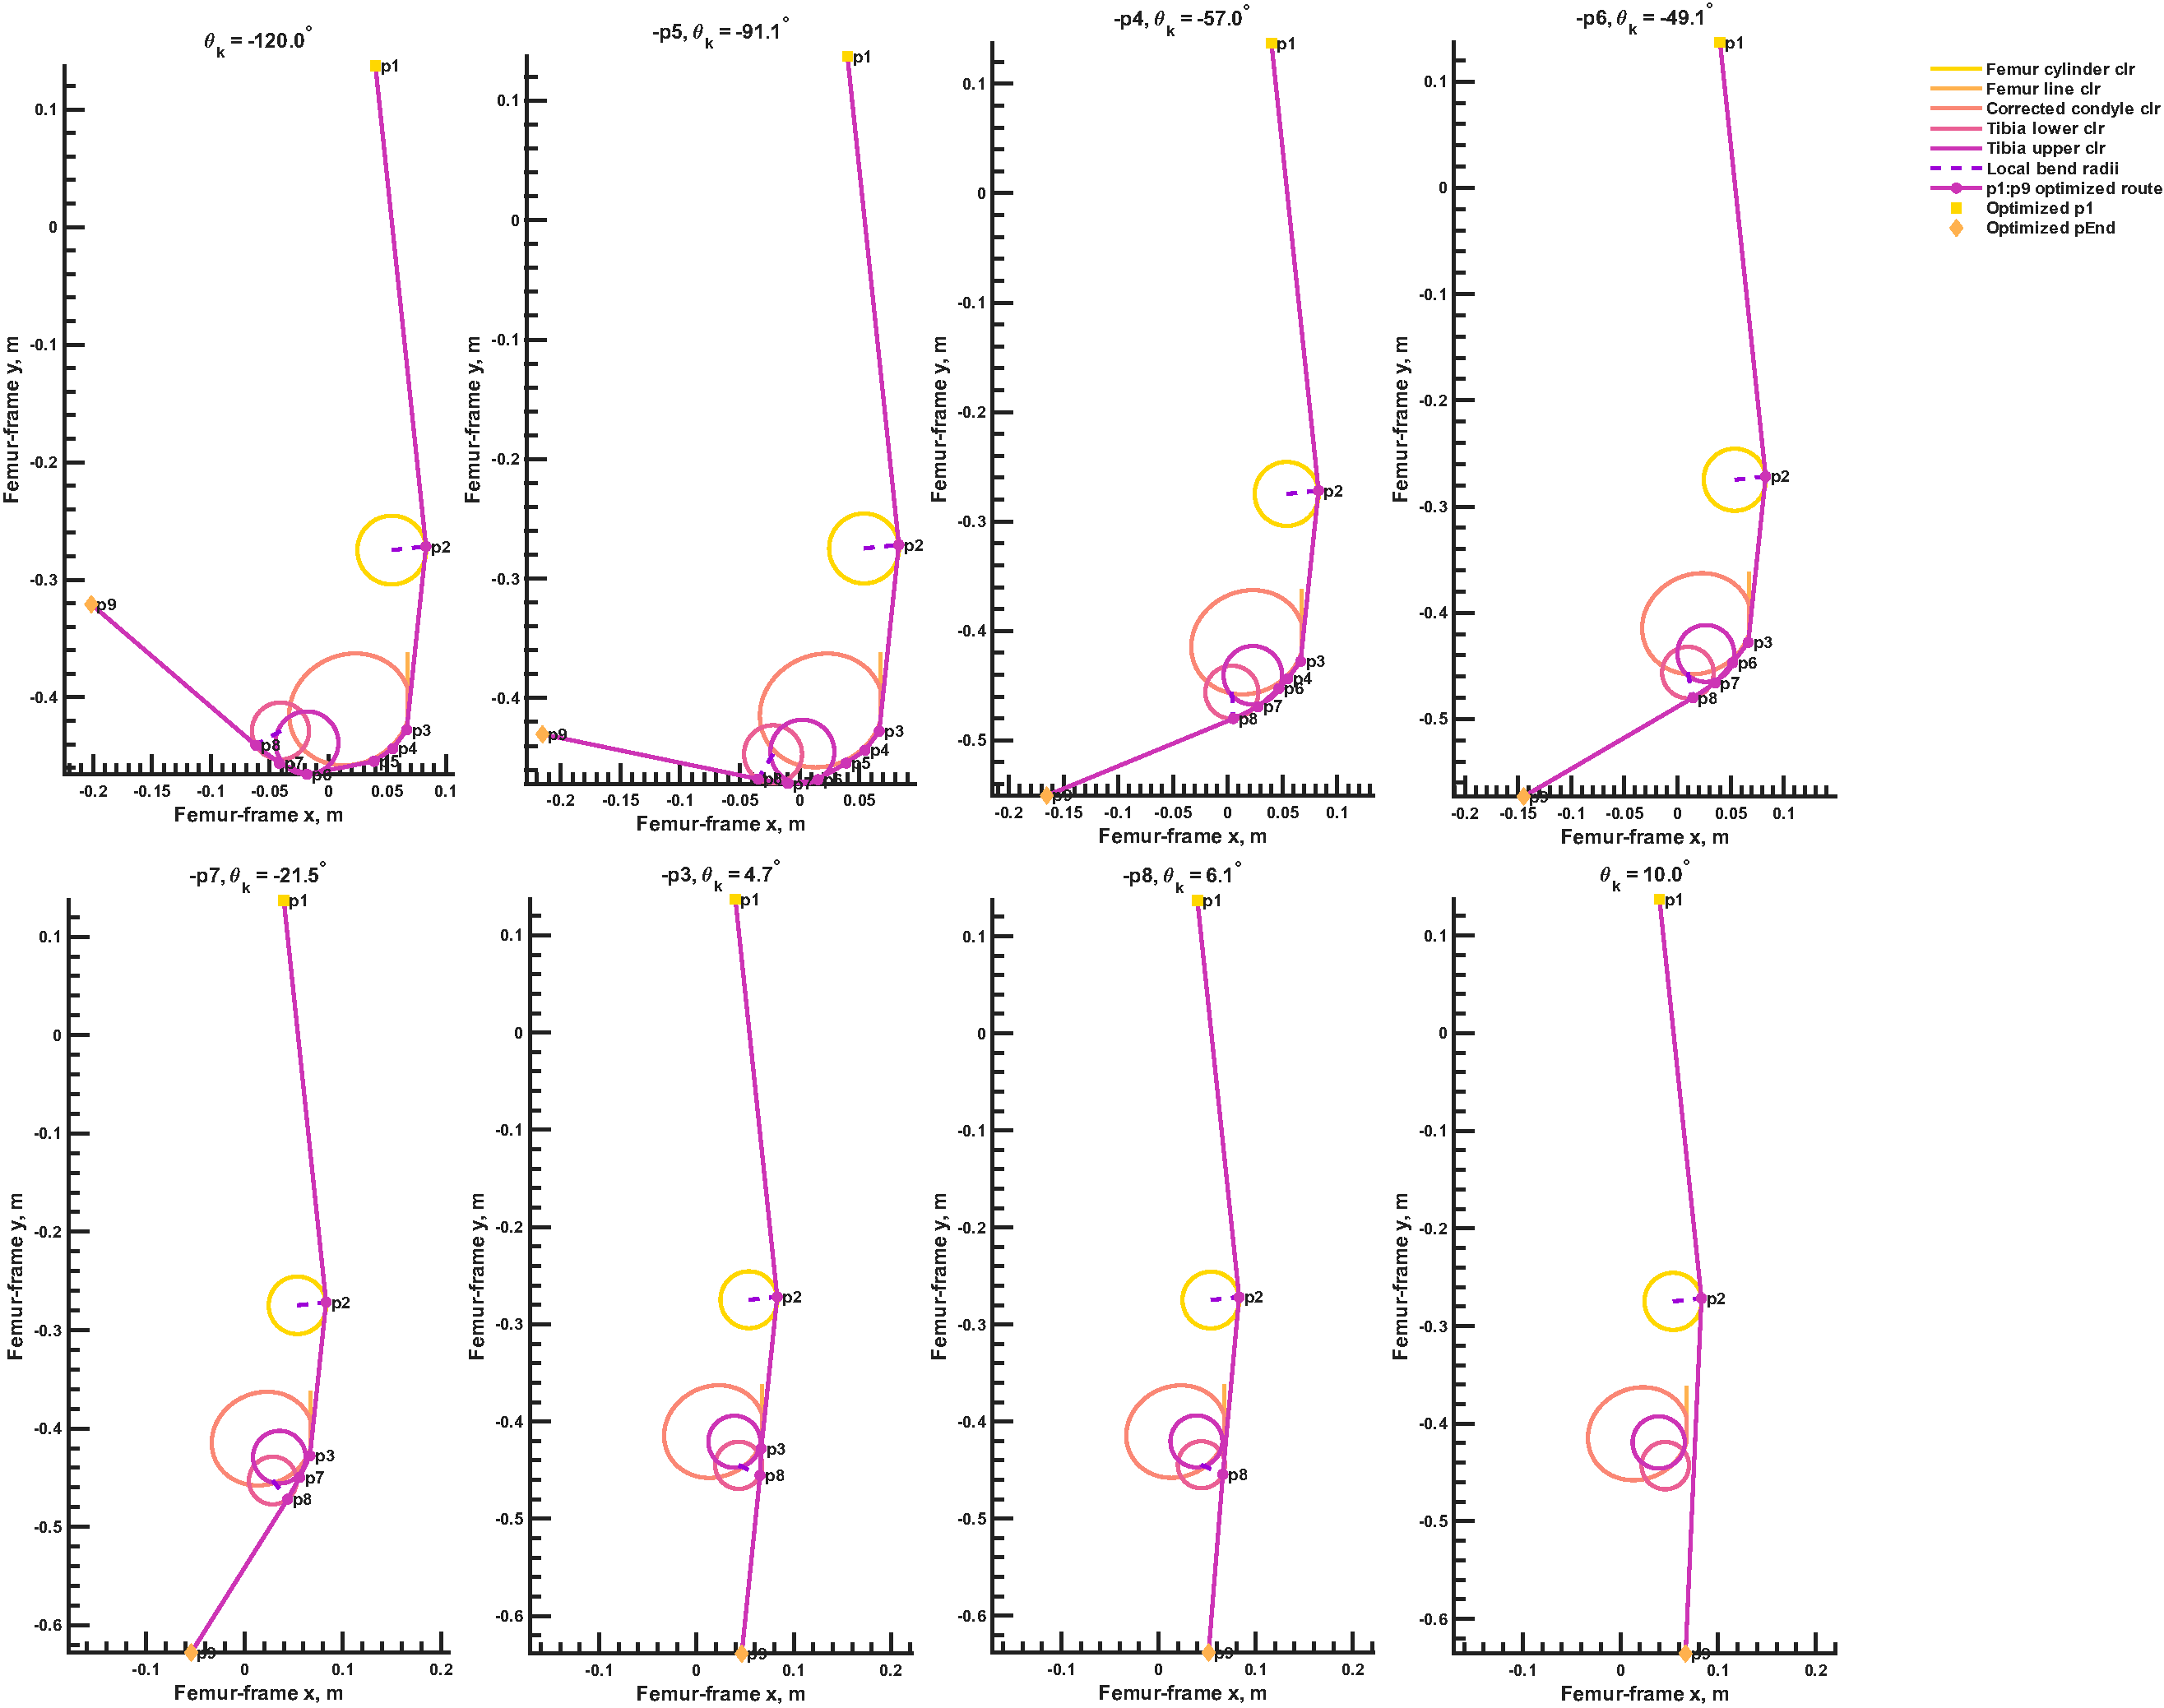
\includegraphics[width=\textwidth]{route_geometry_ext20mm_20260925.pdf}
% ALT TEXT: see route_geometry_ext20mm_20260925.alt.txt beside the figure file.
\caption[Optimized 9-point extensor route geometry at the elimination-event poses]{Eight-panel route-geometry view of the optimized 9-point extensor route of record (\texttt{Vas\_Pam\_20mm\_Result\_20260925.mat}), drawn in the femur frame. Regenerated by \texttt{Export\_AppendixRouteGeo.m}, which ports the plotting block of \texttt{Opt\_run\_Ext.m} verbatim.}
\label{fig:app_route_geometry}
\end{figure}

\begin{figure}[htbp]
\centering
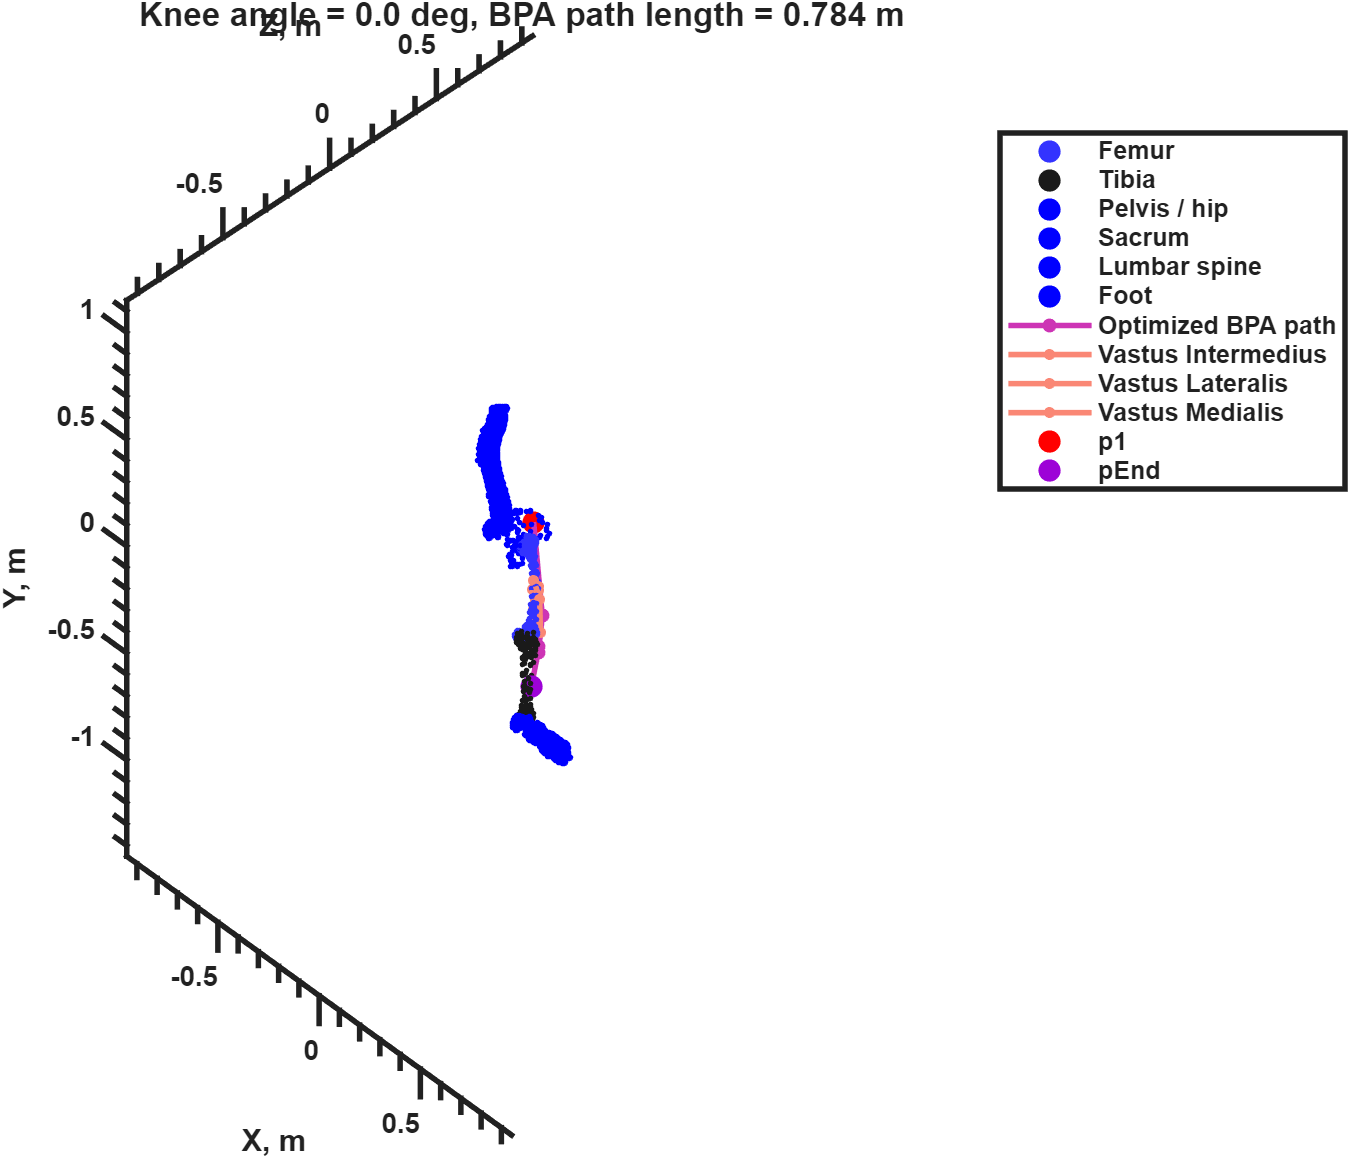
\includegraphics[width=0.85\textwidth]{bone_mesh_static_extensor20mm.png}
% ALT TEXT: see bone_mesh_static_extensor20mm.alt.txt beside the figure file.
\caption[Optimized 20 mm extensor route on the OpenSim bone meshes at zero knee angle]{Static bone-mesh view of the optimized 20 mm extensor route at $\theta_{k}=0^{\circ}$, rendered by \texttt{Export\_AppendixBoneMesh.m}.}
\label{fig:app_bone_mesh}
\end{figure}

\section{Supporting Route Searches and Transmission Sweeps}\label{sec:app_routing_extensions}

The following diagnostics describe earlier optimizer runs and integration status. The five-site batch table concerns the original unity-transmission search; it is distinct from the subsequent size re-solves plotted below. Objective values from different formulations are not directly comparable.

The route redesign of Section~\ref{sec:ongoing} placed both \qty{20}{\mm} actuators on direct attachment routes. The Mono/Bi-pulley algorithms extend that search space by allowing the artificial tendon to be reeved over pulleys before insertion, and the flexor pulley run quantifies what the added routing freedom is worth on the knee-flexor route. The pulley variant converged to a collision-feasible layout with zero bound violations (pattern-search exit flag 1) at an objective of 0.08465 under its own objective function, which differs from the direct route's objective of 74.47, so the two values are not commensurable. The best configuration on file reeves the two actuators over a single tackle-line part at a gain fixed at 1:1, so the pulley acts as a redirect rather than a force multiplier; even so, the redirect alone deepened the peak predicted flexion torque from \qty{81.23}{\newton\cdot\meter} to \qty{85.74}{\newton\cdot\meter}, a gain of \qty{4.51}{\newton\cdot\meter} (\qty{5.6}{\percent}), while holding the off-axis torque to at most \qty{0.803}{\newton\cdot\meter}, under \qty{1}{\percent} of the peak on-axis value; the predicted peaks of the direct and pulley routes exceed the human flexor torque scale of \qty{23.16}{\newton\cdot\meter} by factors of 3.51 and 3.70. The Bi-pulley batch establishes where that freedom runs out on anatomical routes. Across the five OpenSim muscle sites attempted (soleus, tibialis anterior, rectus femoris, medial gastrocnemius, and biceps femoris short head), every run closed with a nonpositive torque margin (objectives of 0.929 for tibialis anterior, 0.997 for soleus, and 3.42 for rectus femoris with a residual worst-constraint value of 0.242), and the medial-gastrocnemius and biceps-femoris-short-head runs terminated at the infeasibility sentinel (objective 101, worst-constraint value 10, exit flag $-2$). For the four runs that report a finite route-to-route clearance, the binding constraint was geometry rather than torque: minimum pair clearances spanned \qty{4.26}{\mm} to \qty{19.14}{\mm} against the \qty{25}{\mm} separation required between adjacent routes (two \qty{10}{\mm} actuator radii plus a \qty{5}{\mm} bundle margin); the medial-gastrocnemius run records no finite clearance, so its failure rests on the infeasibility sentinel alone. What the two algorithms buy is therefore reach and screening: the mono-pulley converts routing freedom into \qty{4.51}{\newton\cdot\meter} of additional predicted flexion torque without mechanical advantage and with off-axis torque below \qty{1}{\percent} of the peak, and the bi-pulley sweep screens candidate anatomical sites, showing that its reeved routes do not yet fit these corridors and redirecting the design effort toward clearance-relaxed attachment sites. These pulley solutions are optimizer-stage results; they have not yet been propagated into the OpenSim or MuJoCo model trees used for the simulation work of Sections~\ref{sec:preliminary_sim_methods}--\ref{sec:preliminary_sim_results}, and the hardware torque tests of the updated compliant system have begun with the extensor route.

The Bi-pulley batch applied the same reeving freedom to five muscle sites of the robot-body model's OpenSim leg, and all five runs failed the torque requirement, with the medial-gastrocnemius and biceps-femoris-short-head runs terminating at the infeasibility sentinel (Table~\ref{tab:bipulley_batch}). For the biceps femoris short head site, whose torque target is \qty{40.2}{\newton\cdot\meter} at the robot-body model's maximum isometric force of \qty{804}{\N}, the pattern search exited with flag $-2$ and returned the sentinel objective of 101 from an initial objective of 1000; Section~\ref{sec:disc_pulley} reports the per-run objectives and the clearance constraints behind these outcomes.

\begin{table}[htbp]
\caption{Bi-pulley batch on five muscle sites of the robot-body model's OpenSim leg. Objective 101 is the batch's infeasibility sentinel; all five runs closed with a nonpositive torque margin. The soleus and tibialis-anterior runs converged feasibly (pattern-search exit flag 1), and their objectives are the normalized torque shortfalls; the remaining three runs exited with flag $-2$.}
\label{tab:bipulley_batch}
\small\begin{tabularx}{\textwidth}{@{}>{\raggedright\arraybackslash}p{0.22\textwidth}>{\raggedright\arraybackslash}p{0.32\textwidth}>{\raggedright\arraybackslash}X@{}}
\toprule
\textbf{Muscle site} & \textbf{Objective} & \textbf{Outcome} \\
\midrule
soleus                    & 0.9968                                       & converged (flag 1), nonpositive torque margin \\
tibialis anterior         & 0.9288                                       & converged (flag 1), nonpositive torque margin \\
rectus femoris            & 3.423 (worst constraint 0.2423)              & nonpositive torque margin \\
medial gastrocnemius      & 101, infeasibility sentinel (worst constraint 10) & pattern-search exit flag $-2$ \\
biceps femoris short head & 101, infeasibility sentinel (worst constraint 10) & pattern-search exit flag $-2$ \\
\bottomrule
\end{tabularx}
\end{table}

The robot-body model itself carries one update from this work. The adductor magnus attachment point P2 was restored to its full-precision location $(-0.1357, -0.0929, 0.0591)$~m, displacing a rounded copy that was disqualified for producing a zero-length via point that nullified the flexion torque; the regenerated mirrored model passed its validation with zero non-mirrored pairs. At the restored location, the muscle delivers \qty{34.28}{\newton\cdot\meter} of flexion torque, $1.12\times$ the human target of \qty{30.61}{\newton\cdot\meter}, and \qty{27.62}{\newton\cdot\meter} of adduction torque, $0.82\times$ the human target of \qty{33.60}{\newton\cdot\meter}. These redesigned routes remain optimizer-stage results: the robot-body OpenSim model contains no pulley entities, and no via points or markers were added to it for these routes (its eight pre-existing moving-path-point vias, the rectus-femoris and vastii patella-tracking points, one per muscle per leg, belong to the original muscle paths). The MuJoCo conversion used for the simulation work predates the pulley batch and the adductor-magnus restoration, so it carries one stale path point, the pre-restoration rounded adductor-magnus P2. Physical torque tests of the redesigned routes have begun (Section~\ref{sec:disc_pulley}).

The same redesign pipeline was then extended from the knee to all 27 muscle-actuators of the robot-body model, and this whole-body extension is reported as work in progress rather than a completed result. The first pass reached 19 of the 27 actuators before the run stopped, and its chosen solutions showed that the penalty-based formulation itself was the binding limitation: all but one of the chosen routes violated the feasibility constraints, the sole exception being the biceps femoris long-head pair, whose worst-angle margin of $+0.03\,\%$ is indistinguishable from zero. The formulation was then restructured so that the task envelope, the joint-angle window each route must serve, acts as a hard feasible set rather than a penalty. In the restructured pass, twelve of the 27 actuators terminated on a concatenation error in the route builder (the three lumbar-wall actuators, tibialis posterior, the seven distal-foot actuators, and adductor magnus), leaving fifteen finalized routes. Eight of the fifteen were chosen from constraint-feasible configurations: semimembranosus, biceps femoris long head, tensor fasciae latae, soleus, lateral gastrocnemius, tibialis anterior, iliacus, and psoas. Of those eight, six also met the torque requirement at every angle, with worst-angle margins spanning $+0.25\,\%$ (biceps femoris long head) to $+250.7\,\%$ (tensor fasciae latae); the semimembranosus and soleus routes satisfy the geometry but remain short of their torque targets. The crash set and the two torque-short feasible routes define the remaining engineering: the route builder needs a fix for the concatenation failure, and the short routes need either larger actuators or relaxed corridors.

The unadjusted cam optimizer solution had minimum margins of $+31.30$\,\% against the required envelope and $+42.34$\,\% against the plain human target; the adjusted design used in Chapter~\ref{ch:torque} has margins of $+30.83$\,\% and $+39.77$\,\%, respectively.

\begin{figure}[p]
\centering
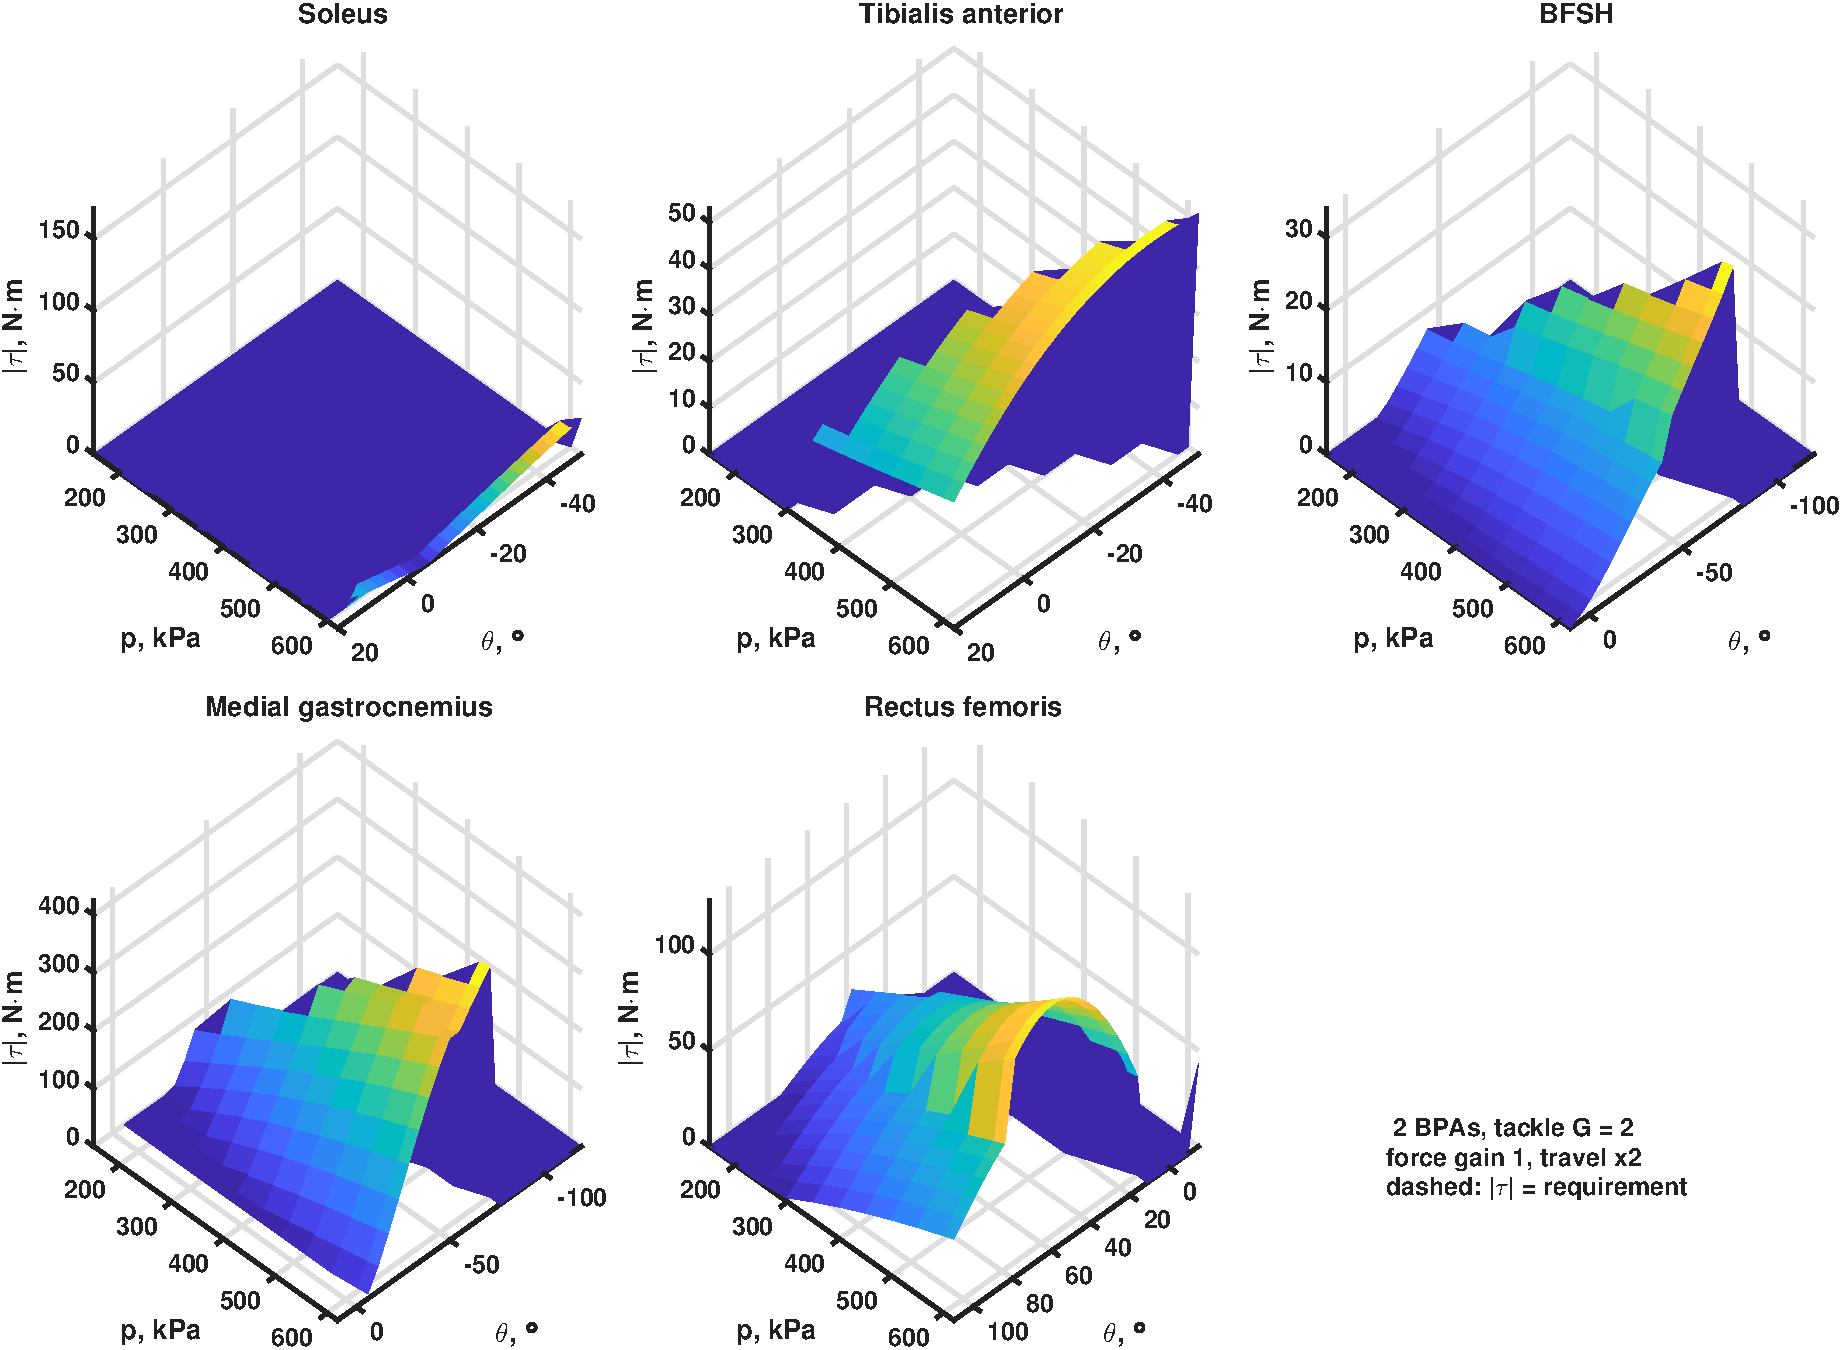
\includegraphics[width=\textwidth]{pulley_torque_resolved.pdf}
\caption{Predicted insertion-torque magnitude versus joint angle and supply pressure for two BPAs through a two-part tackle (force gain 1, travel gain 2), with actuator sizes re-solved. Panels show soleus, tibialis anterior, biceps femoris short head (BFSH), medial gastrocnemius with ankle fixed at zero, and rectus femoris evaluated at the hip. Dashed curves mark equality with the maximum-isometric OpenSim requirement; no equality curve lies within the soleus panel.}
\label{fig:PulleySurfaces}
\end{figure}

\begin{figure}[p]
\centering
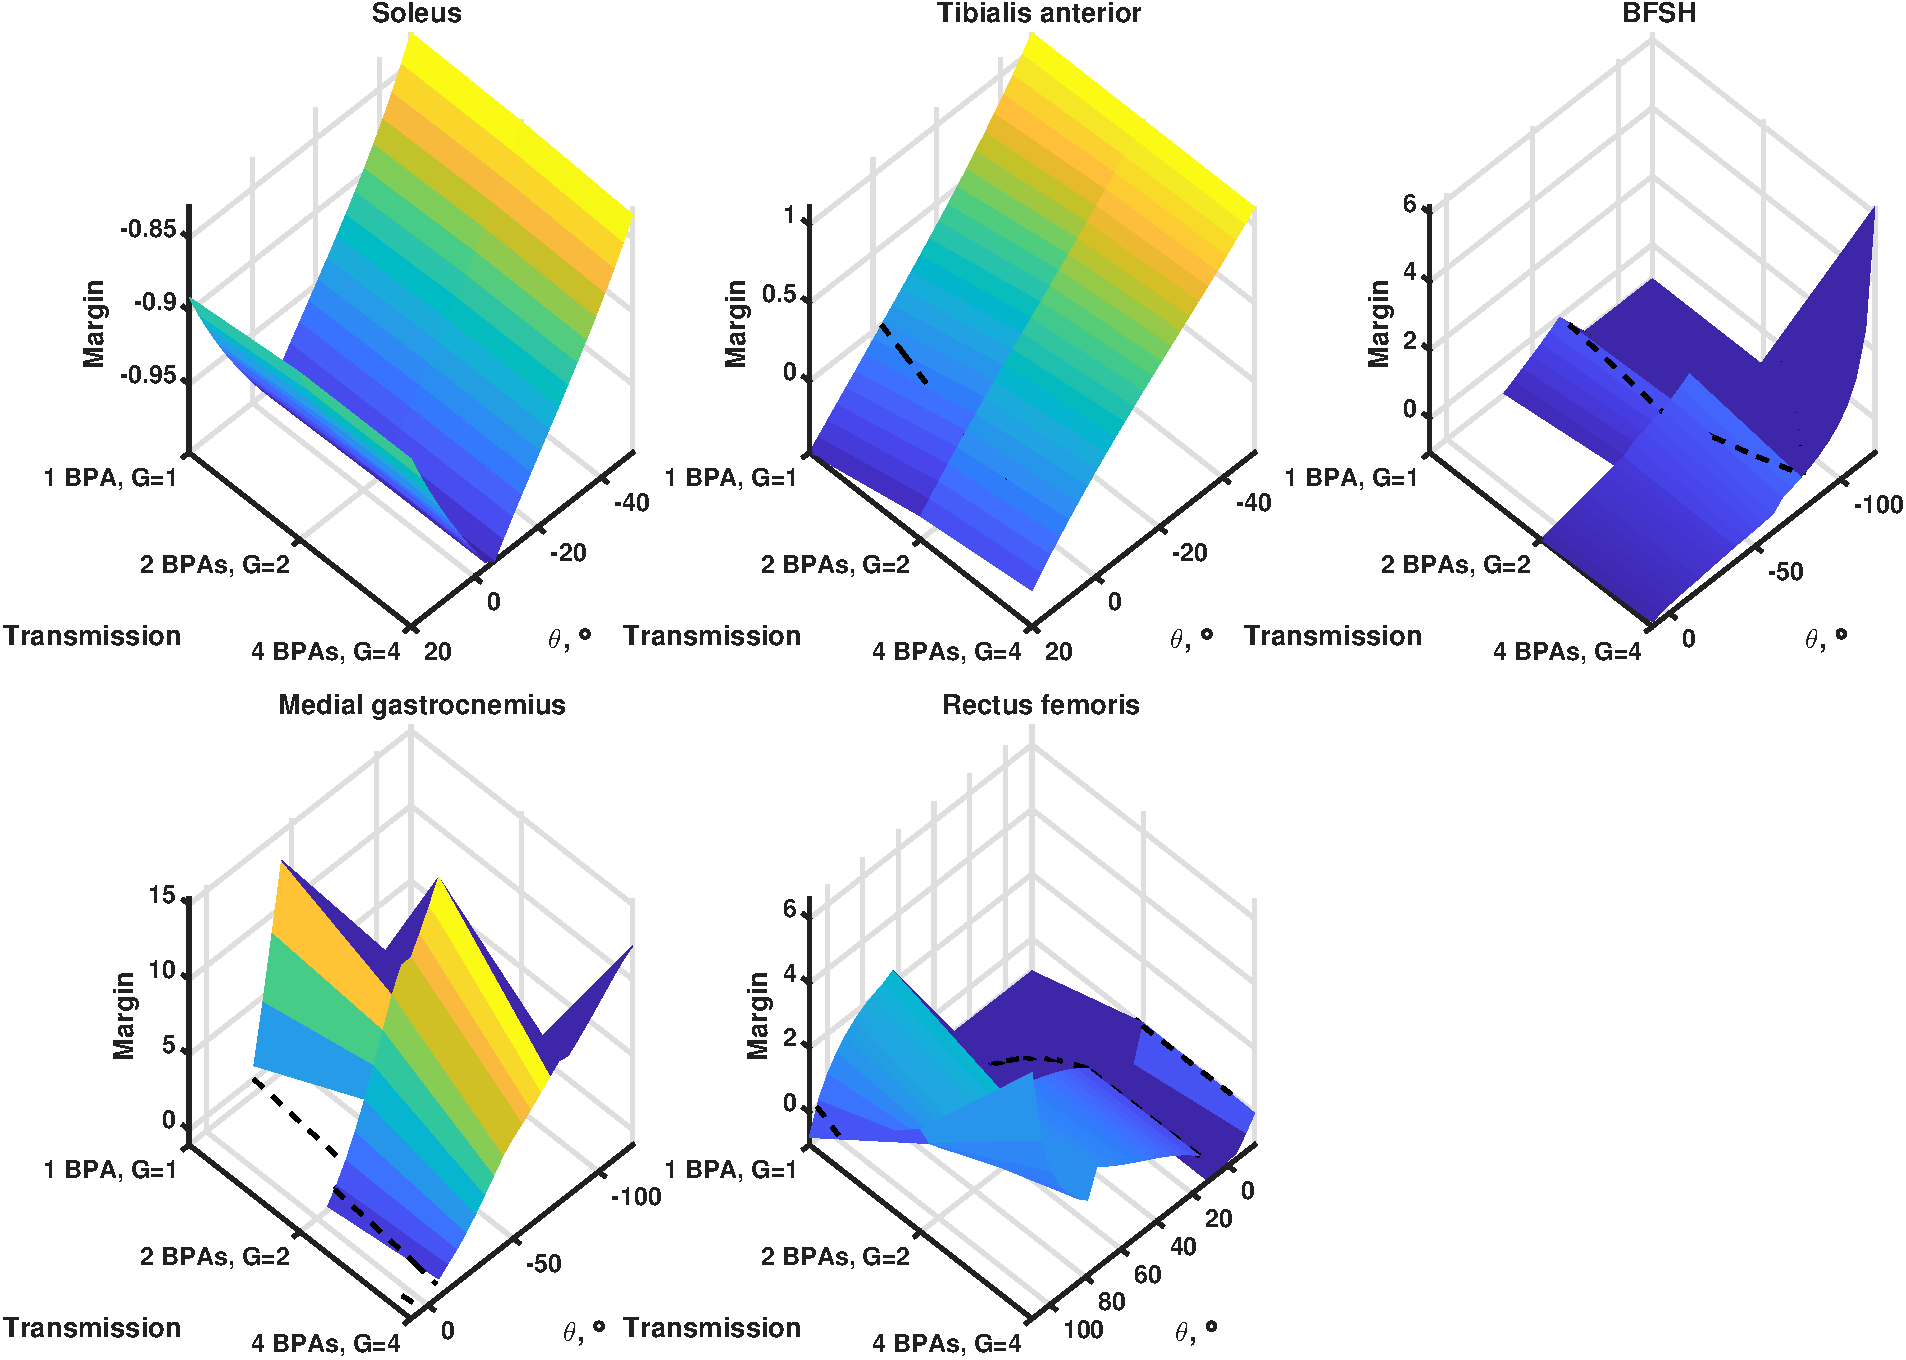
\includegraphics[width=\textwidth]{pulley_margin_resolved.pdf}
\caption{Torque margins at \qty{620}{\kPa} for the single-BPA baseline, two BPAs through a two-part tackle, and four BPAs through a four-part tackle. Actuator sizes are re-solved for each configuration. A positive fractional margin exceeds the maximum-isometric OpenSim requirement; the dashed line marks zero. Panels and evaluation planes follow Figure~\ref{fig:PulleySurfaces}.}
\label{fig:PulleyMargins_resolved}
\end{figure}

\clearpage
\begin{figure}[htbp]
\centering
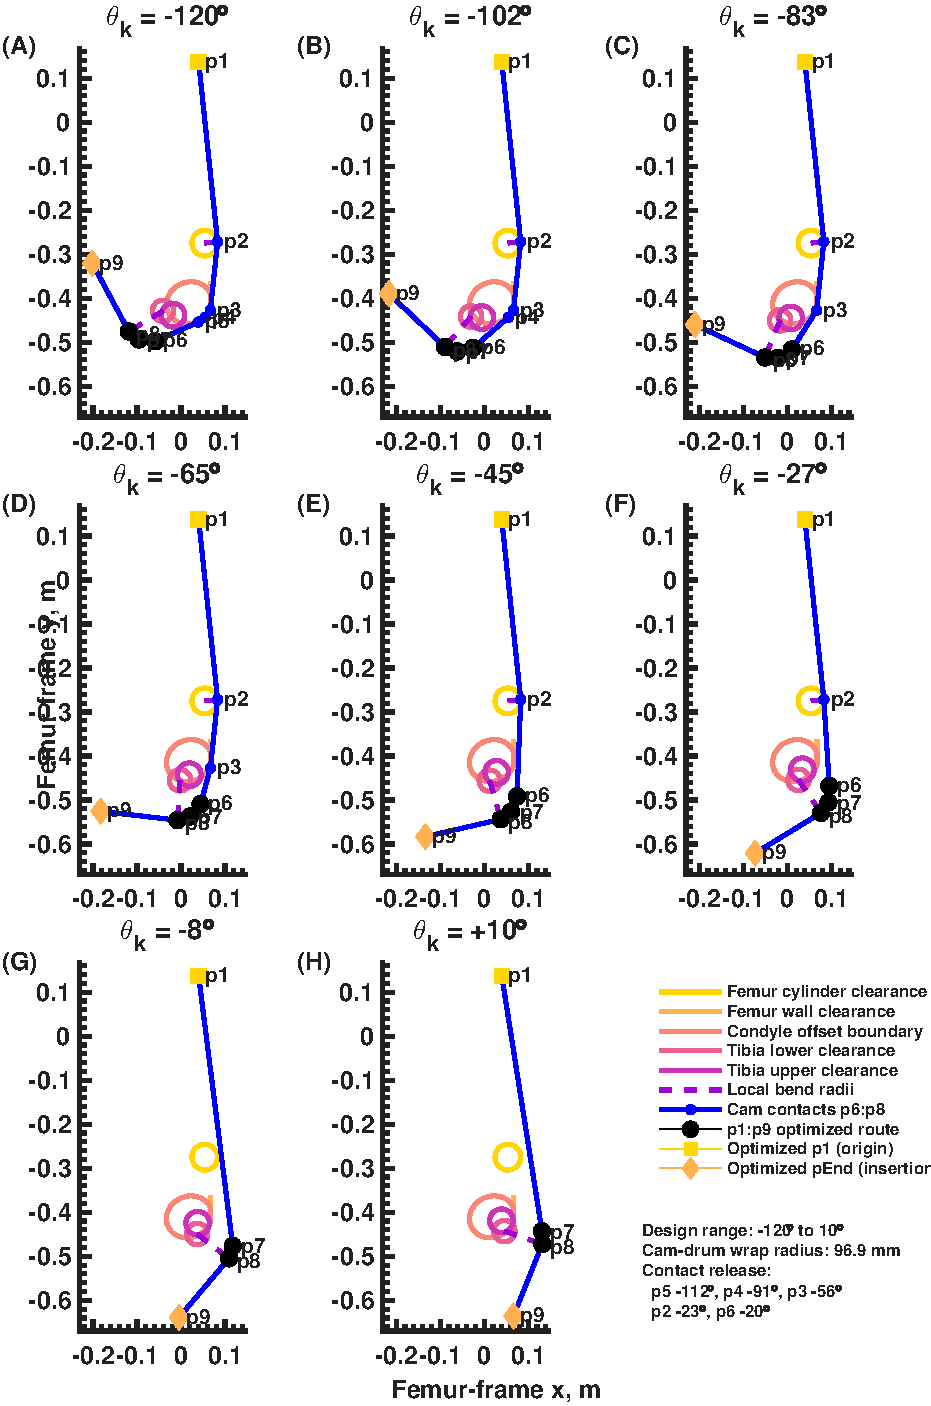
\includegraphics[width=\textwidth,trim=0.000bp 237.500bp 0.000bp 0.000bp,clip]{extensor_cam_route.pdf}
\caption{Cam-extensor poses A--F, spanning \ang{-120} to \ang{-27}. Blue lines show the route; colored outlines show the clearance envelopes. The remaining poses and original legend are in Figure~\ref{fig:app_cam_GH}.}
\label{fig:app_cam_AF}
\end{figure}

\begin{figure}[htbp]
\centering
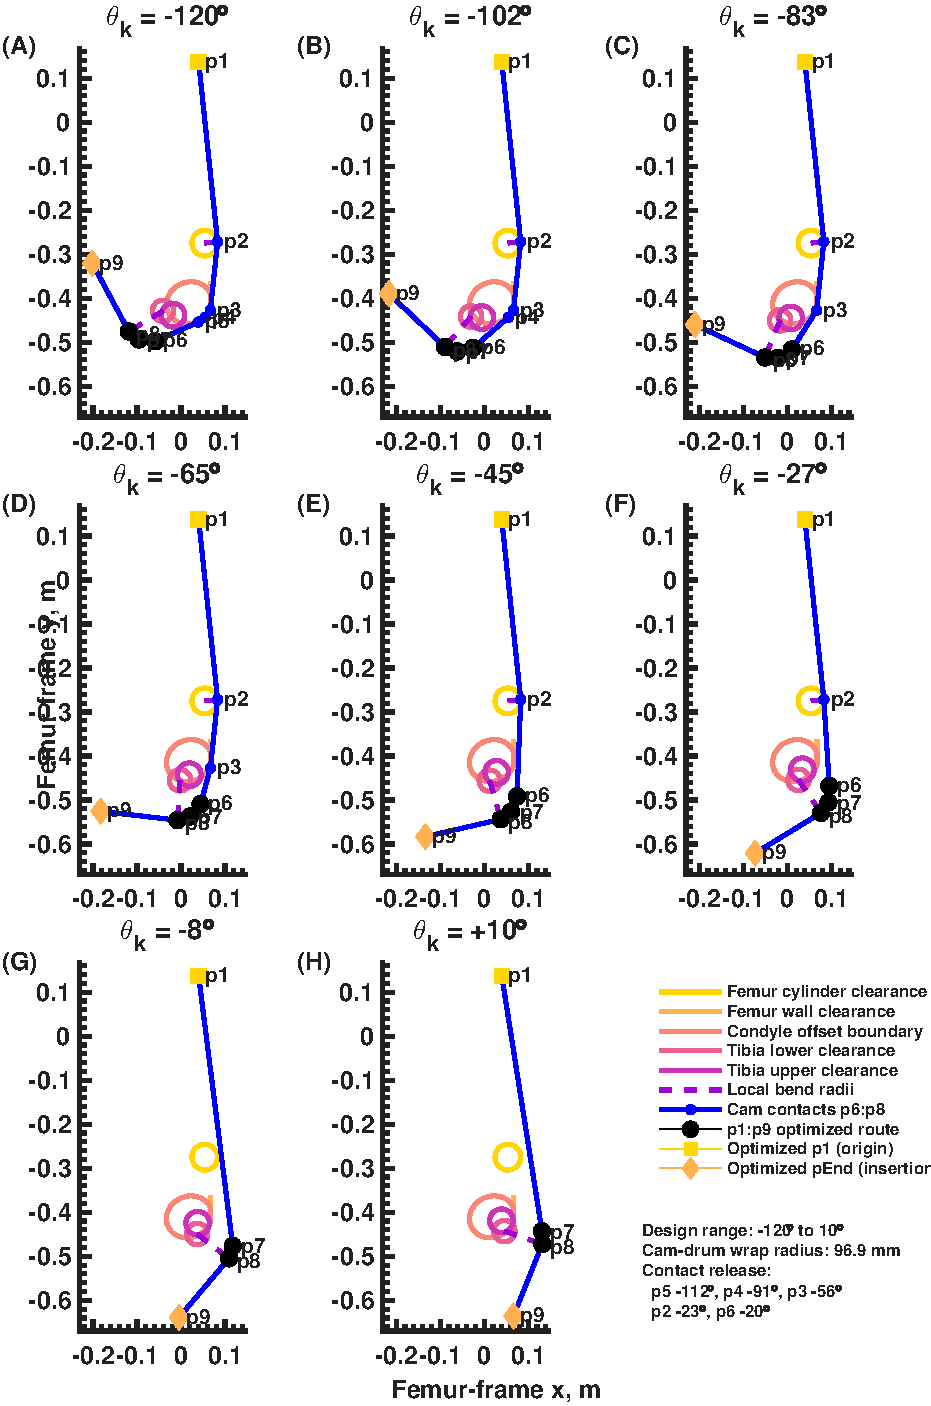
\includegraphics[width=\textwidth,trim=0.000bp 0.000bp 0.000bp 437.500bp,clip]{extensor_cam_route.pdf}
\caption{Cam-extensor poses G and H at \ang{-8} and \ang{10}, with the original legend, \qty{96.9}{\mm} cam-drum radius, and contact-release schedule. Panel letters continue Figure~\ref{fig:app_cam_AF}.}
\label{fig:app_cam_GH}
\end{figure}
\clearpage

\section{Supporting Torque-Prediction Fit Statistics}\label{sec:app_torque_fit_details}

The earlier cross-configuration fit below is distinct from the adopted two-stage identification. The pre-optimization comparison and the adopted pinned-flexor and pinned-extensor per-test fits appear in Chapter~\ref{ch:torque} (Tables~\ref{tab:FlxPinPreGof}, \ref{tab:FlxPinGof}, and~\ref{tab:ExtPinGof}).







\begin{table}[p]
\centering\small
\caption{Goodness of fit for the improved torque model across test configurations. RMSE and maximum absolute residual are in $\text{N}\cdot\text{m}$.}
\label{tab:TorqueFit}
\begin{tabularx}{\textwidth}{@{}>{\raggedright\arraybackslash}p{0.55\textwidth}*{3}{>{\centering\arraybackslash}X}@{}}
\toprule
\textbf{Configuration} & \textbf{RMSE} & \textbf{FVU} & \textbf{Max.\ residual} \\
\midrule
Flexor, pin joint, $l_{0}=\qty{48.5}{\cm}$ (training) & 1.616 & 0.0958 & 3.2527 \\
Flexor, pin joint, $l_{0}=\qty{45.7}{\cm}$ (validation) & 2.1214 & 0.0878 & 5.1690 \\
Extensor, biomimetic knee, $l_{0}=\qty{51.8}{\cm}$ & 0.8920 & 0.3396 & 1.4188 \\
Flexor, biomimetic knee, $\diameter$\qty{10}{\mm}, $l_{0}=\qty{41.5}{\cm}$ & 0.3007 & 0.0102 & 0.4647 \\
Flexor, biomimetic knee, $\diameter$\qty{20}{\mm}, $l_{0}=\qty{41.5}{\cm}$ (\qty{620}{\kPa}) & 1.8024 & 0.0499 & 3.5678 \\
\bottomrule
\end{tabularx}
\end{table}
